%File: formatting-instructions-latex-2024.tex
%release 2024.0
\documentclass[letterpaper]{article} % DO NOT CHANGE THIS
\usepackage{aaai24}  % DO NOT CHANGE THIS
\usepackage{times}  % DO NOT CHANGE THIS
\usepackage{helvet}  % DO NOT CHANGE THIS
\usepackage{courier}  % DO NOT CHANGE THIS
\usepackage[hyphens]{url}  % DO NOT CHANGE THIS
\usepackage{graphicx} % DO NOT CHANGE THIS
\urlstyle{rm} % DO NOT CHANGE THIS
\def\UrlFont{\rm}  % DO NOT CHANGE THIS
\usepackage{natbib}  % DO NOT CHANGE THIS AND DO NOT ADD ANY OPTIONS TO IT
\usepackage{caption} % DO NOT CHANGE THIS AND DO NOT ADD ANY OPTIONS TO IT
\frenchspacing  % DO NOT CHANGE THIS
\setlength{\pdfpagewidth}{8.5in}  % DO NOT CHANGE THIS
\setlength{\pdfpageheight}{11in}  % DO NOT CHANGE THIS
%
% These are recommended to typeset algorithms but not required. See the subsubsection on algorithms. Remove them if you don't have algorithms in your paper.
\usepackage{algorithm}
\usepackage{algorithmic}



\usepackage{amsmath}
\usepackage{epsfig}
\usepackage{graphicx}
\usepackage{amssymb}
%\usepackage{fullpage}
\usepackage{fancyhdr}
\usepackage{booktabs}
\usepackage{multirow}
\usepackage[T1]{fontenc}
%\usepackage[ruled,vlined]{algorithm2e}
%\usepackage{algorithmic}
\usepackage{subfigure}



%
% These are are recommended to typeset listings but not required. See the subsubsection on listing. Remove this block if you don't have listings in your paper.
\usepackage{newfloat}
\usepackage{listings}
\DeclareCaptionStyle{ruled}{labelfont=normalfont,labelsep=colon,strut=off} % DO NOT CHANGE THIS
\lstset{%
	basicstyle={\footnotesize\ttfamily},% footnotesize acceptable for monospace
	numbers=left,numberstyle=\footnotesize,xleftmargin=2em,% show line numbers, remove this entire line if you don't want the numbers.
	aboveskip=0pt,belowskip=0pt,%
	showstringspaces=false,tabsize=2,breaklines=true}
\floatstyle{ruled}
\newfloat{listing}{tb}{lst}{}
\floatname{listing}{Listing}
%
% Keep the \pdfinfo as shown here. There's no need
% for you to add the /Title and /Author tags.

% DISALLOWED PACKAGES
% \usepackage{authblk} -- This package is specifically forbidden
% \usepackage{balance} -- This package is specifically forbidden
% \usepackage{color (if used in text)
% \usepackage{CJK} -- This package is specifically forbidden
% \usepackage{float} -- This package is specifically forbidden
% \usepackage{flushend} -- This package is specifically forbidden
% \usepackage{fontenc} -- This package is specifically forbidden
% \usepackage{fullpage} -- This package is specifically forbidden
% \usepackage{geometry} -- This package is specifically forbidden
% \usepackage{grffile} -- This package is specifically forbidden
% \usepackage{hyperref} -- This package is specifically forbidden
% \usepackage{navigator} -- This package is specifically forbidden
% (or any other package that embeds links such as navigator or hyperref)
% \indentfirst} -- This package is specifically forbidden
% \layout} -- This package is specifically forbidden
% \multicol} -- This package is specifically forbidden
% \nameref} -- This package is specifically forbidden
% \usepackage{savetrees} -- This package is specifically forbidden
% \usepackage{setspace} -- This package is specifically forbidden
% \usepackage{stfloats} -- This package is specifically forbidden
% \usepackage{tabu} -- This package is specifically forbidden
% \usepackage{titlesec} -- This package is specifically forbidden
% \usepackage{tocbibind} -- This package is specifically forbidden
% \usepackage{ulem} -- This package is specifically forbidden
% \usepackage{wrapfig} -- This package is specifically forbidden
% DISALLOWED COMMANDS
% \nocopyright -- Your paper will not be published if you use this command
% \addtolength -- This command may not be used
% \balance -- This command may not be used
% \baselinestretch -- Your paper will not be published if you use this command
%  -- No page breaks of any kind may be used for the final version of your paper
% \columnsep -- This command may not be used
%  -- No page breaks of any kind may be used for the final version of your paper
% \pagebreak -- No page breaks of any kind may be used for the final version of your paperr
% \pagestyle -- This command may not be used
% \tiny -- This is not an acceptable font size.
% \vspace{- -- No negative value may be used in proximity of a caption, figure, table, section, subsection, subsubsection, or reference
% \vskip{- -- No negative value may be used to alter spacing above or below a caption, figure, table, section, subsection, subsubsection, or reference

\setcounter{secnumdepth}{0} %May be changed to 1 or 2 if section numbers are desired.

% The file aaai24.sty is the style file for AAAI Press
% proceedings, working notes, and technical reports.
%

% Title

% Your title must be in mixed case, not sentence case.
% That means all verbs (including short verbs like be, is, using,and go),
% nouns, adverbs, adjectives should be capitalized, including both words in hyphenated terms, while
% articles, conjunctions, and prepositions are lower case unless they
% directly follow a colon or long dash

\title{Bias-Conflict Sample Synthesis and Adversarial Removal Debias Strategy for Temporal Sentence Grounding in Video}
%\title{\fontsize{14}{16}{\centering{Bias-Conflict Sample Synthesis and Adversarial Removal Debias Strategy for Temporal Sentence Grounding in Video}}}


\author{
	Zhaobo Qi\textsuperscript{\rm 1},
	Yibo Yuan\textsuperscript{\rm 1},
	Xiaowen Ruan\textsuperscript{\rm 1},
	Shuhui Wang\textsuperscript{\rm 2}, \\
	Weigang Zhang\textsuperscript{\rm 1}\thanks{Corresponding author.},
	Qingming Huang\textsuperscript{\rm 2, \rm 3 *}
}
\affiliations {
	\textsuperscript{\rm 1}Harbin Institute of Technology, Weihai, China\\
	\textsuperscript{\rm 2}Key Lab of Intell. Info. Process., Inst. of Comput. Tech., CAS, Beijing, China\\
	\textsuperscript{\rm 3}University of Chinese Academy of Sciences, Beijing, China\\
	%\textsuperscript{\rm 4}Peng Cheng Laboratory, Shenzhen, China\\
	qizb@hit.edu.cn, \{yuanyibo21,22s130489\}@stu.hit.edu.cn, wangshuhui@ict.ac.cn, \\ wgzhang@hit.edu.cn, qmhuang@ucas.ac.cn
}


% REMOVE THIS: bibentry
% This is only needed to show inline citations in the guidelines document. You should not need it and can safely delete it.
\usepackage{bibentry}
% END REMOVE bibentry

\begin{document}

\maketitle

\begin{abstract}
	Temporal Sentence Grounding in Video (TSGV) is troubled by dataset bias issue, which is caused by the uneven temporal distribution of the target moments for samples with similar semantic components in input videos or query texts. Existing methods resort to utilizing prior knowledge about bias to artificially break this uneven distribution, which only removes a limited amount of significant language biases. In this work, we propose the bias-conflict sample synthesis and adversarial removal debias strategy (BSSARD), which dynamically generates bias-conflict samples by explicitly leveraging potentially spurious correlations between single-modality features and the temporal position of the target moments. Through adversarial training, its bias generators continuously introduce biases and generate bias-conflict samples to deceive its grounding model. Meanwhile, the grounding model continuously eliminates the introduced biases, which requires it to model multi-modality alignment information. BSSARD will cover most kinds of coupling relationships and disrupt language and visual biases simultaneously. Extensive experiments on Charades-CD and ActivityNet-CD demonstrate the promising debiasing capability of BSSARD. Source codes are available at~\url{https://github.com/qzhb/BSSARD}.
\end{abstract}



Federated learning (FL) \cite{mcmahan2017communication, kairouz2021advances} recently emerged in response to the challenges in data privacy, storage cost and computation commonly faced by the conventional (centralized) learning systems. In centralized learning, a server collects and stores data to be used for model training, raising concerns regarding potential leakage of sensitive information and inefficient utilization of the storage and computation resources. Lately, advancements in software and hardware technologies have equipped smart edge devices with computational power that enables local data processing, allowing implementation of distributed frameworks such as FL in a variety of real-world applications \cite{chen2019communication}. In FL systems, participating devices collaboratively learn a model while preserving privacy by training on local data that remains private. A server aggregates local updates to obtain a global model which is then distributed to the clients; in turn, the clients continue local training using the latest global model as a starting point. In addition to the conventional supervised learning, federated learning is suitable for meta-learning and unsupervised learning problems \cite{jiang2019improving, servetnyk2020unsupervised}. 

Heterogeneity in local data distribution, as well as imbalance in the computation and memory capabilities of the participating devices, present major challenges to federated learning \cite{zhao2018federated, yoon2022bitwidth}. Practical scenarios where both sources of heterogeneity occur include healthcare disorder prediction for patients with different profiles and monitoring devices, transportation systems over different vehicles and terrain, and indoor/outdoor air quality detection, to name just a few. Several recent FL techniques aim to 
alleviate the impact of data, model or device heterogeneity \cite{jiang2020federated, lin2020ensemble, diao2020heterofl, wang2022does}. However, variations in bitwidth available to the clients that participate in training have been much
less studied \cite{yoon2022bitwidth}. To our knowledge, there exists no prior work in literature investigating FL in 
setting where both the local data and device bitwidth are heterogeneous -- the focus of our work.

%While prior work has not explored solution to the problem on both bitwidth and data heterogeneity, it is natural in practical applications that clients need to train local models in both heterogeneity. We therefore explore the FL problem combining data and bitwidth heterogeneity and address the challenges from both heterogeneity. 

On one hand, clients' devices collect and/or generate data at different times and locations, leading to discrepancy in data amounts and distribution. When distributed devices train locally, each learned model optimizes an objective specified in regard to a local dataset. If the data across participating devices is non-IID, the devices end up optimizing distinct objectives which generally adversely affects 
training convergence and, ultimately, negatively impacts performance of the resulting global model trained by classical FL algorithms such as FedAvg \cite{mcmahan2017communication, li2019convergence}. This is exacerbated when a client's dataset contains only a small subset of classes or few data points, leading to an insufficiently expressive local model. In turn, using such models in the aggregation step at the server leads to a global model that lacks robustness and in general may significantly underperform its centrally trained counterparts \cite{zhao2018federated}.

On the other hand, to satisfy the constraints on local compute and memory footprint as well as on the communication bandwidth between clients and the central server, each client needs to train a local model in low bitwidth operations and store the updated model in low bitwidth \cite{yoon2022bitwidth}. When the clients' devices have different bitwidth capabilities, a number of novel challenges arise including: (1) Quantized training conducted at lower precision levels does not necessarily lead to expressive local model; (2) the server needs to aggregate local models that are represented by different number of bits; and (3) following the aggregation of local updates, the server should communicate to clients the new global model re-quantized at levels matching the capabilities of different devices. Prior works that deploy model compression in distributed settings focus on reducing the communication cost \cite{reisizadeh2020fedpaq, chen2021communication, chen2021decentralized}; those methods utilize full precision weights in the training process rather than trying to train under weight precision constraint. To address the problem of aggregating models trained at different precision, \cite{yoon2022bitwidth} proposed a progressive weight de-quantizer that transforms low precision models to their full precision versions before aggregating them. The de-quantizer there requires the server to train DenseNet for de-quantizing low precision models; the method assumes the local data distribution is the same across different clients and thus does not apply to the heterogeneous data settings studied in this paper.
%; however, the re-quantized models are not personalized to clients' data distribution. 
Note that all of these methods are restricted to supervised learning.

The contributions of this paper are summarized as follows:

\begin{enumerate}

\item For the first time, a novel FL problem characterized by heterogeneous local data distributions and varied capabilities of clients' devices is studied.
This is the first work to consider the non-trivial task of aggregating models which due to varied bitwidth and heterogeneous data have incompatible parameters and different expressiveness.
While prior work addresses either source of heterogeneity in isolation of the other, to our knowledge the combination of the two has not been investigated previously. Indeed, new challenges set forth by the combination of the heterogeneity sources render the prior techniques ineffective.

\item We present a new FL framework, Fed-QSSL, that enables learning personalized and robust low-bitwidth models in settings characterized by diverse infrastructure and data distributions. Fed-QSSL combines low-bitwidth quantization training with self-supervised 
learning at the client side, and deploys de-quantization, weighted aggregation and re-quantization at the 
server side.

\item We theoretically analyze the impact of low-bit training on the convergence and robustness of learned
models. In particular, we present a bound on the variance of the quantization errors in local and global training and investigate the associated convergence speed. The analysis demonstrates that low-bit training with 
Fed-QSSL on heterogeneous data allows learning meaningful representations. 

\item Finally, the efficacy of the proposed algorithm is tested in a variety of experiments.

\end{enumerate}

\subsection{Related work}

{\bf Bitwidth heterogeneity in FL.} To address local infrastructure constraints, \cite{diao2020heterofl} rely
on models with simple architectures and low-bit parameter representation. However, existing prior work
typically assumes that clients train models of same precision, e.g., the same bitwidth, which may often
be violated in practice since the participating devices generally have different computational power and/or memory 
footprint. The varying infrastructure capabilities of the clients' devices imply that the models they are able to 
deploy differ in size, i.e., devices with more computational power and memory allow models of higher 
precision (e.g., 16-bit and 32-bit) while less capable devices may only handle low-precision models (e.g.,
those storing parameters in 2-bit or 4-bit precision). To satisfy local infrastructure constraints, not only should 
a model be represented and stored at reduced precision levels but the training process should also rely on 
operations at such levels (i.e., perform quantized training in low-bitwidth). Recently, \cite{yoon2022bitwidth} 
studied the bitwidth heterogeneity problem in FL and proposed a progressive de-quantization of the received
local models prior to their aggregation into a global model.

{\bf Quantized neural network training.} 
When the compute/storage resources are limited, on-device training of deep neural networks at full precision is rendered infeasible. To this end, recent works have explored model size reduction and the training that leads to low bitwidth weights/activations. These include binarized neural networks (BNN) and XNOR-Net which binarize the weights and activations of convolutional layers to reduce the computation complexity in the forward pass \cite{hubara2017quantized, rastegari2016xnor}.
Specifically, in the forward pass the computationally expensive convolutional operations are implemented via bitwise operation kernels that evaluate the dot product of binary vectors $\x$ and $\mathbf{y}$
%For instance, when the vectors are $1$-bit, the $1$-bit dot product kernel is 
\begin{align*}
    \x \cdot \mathbf{y} = \mathrm{bitcount}(\mathrm{and} (\x, \mathbf{y})), x_i, y_i \in \{0, 1 \} \ \forall i,
\end{align*}
where $\mathrm{bitcount}(\cdot)$ counts the number of bits in its argument. Such a kernel can be generalized to accommodate operations on $M$-bit fixed-point integer sequence $x$ and $K$-bit fixed-point integer sequence $y$, incurring computation complexity of $\O(MK)$ (i.e., the complexity is proportional to the vector bitwidths). Related work \cite{zhou2016dorefa} presents DoReFa-Net which reduces the backpropagation computation cost by quantizing gradients in the backward pass, and studies the effect of the weight, activation and gradient bitwidth choice on the model performance. Subsequent works include techniques that deploy training without floating-point operations, gradient clipping, and training under mixed precision \cite{wen2017terngrad, zhang2017zipml, zhu2020towards, zhang2020fixed}. While all of the aforementioned methods investigate quantization in supervised learning settings, recently there has been interest in quantizing models for self-supervised learning. In \cite{cao2022synergistic}, the authors propose self-supervised and quantization learning (SSQL), which contrasts features learned from the quantized and full precision models in order to provide reasonable accuracy of quantized models and boost the accuracy of the full precision model. While this work can balance the accuracy and bitwidth in resource constrained settings, it still requires full precision operations and gradient storage during training. 

%In the distributed learning setting, the representation learning nature in SSL has motivated a few recent work to look into the efficacy of self supervised learning in learning robust representations from heterogeneous data sources \cite{wang2022does}.

{\bf Non-IID data and distributed self-supervised learning.} There have been multiple efforts to ameliorate the impact of data heterogeneity on the performance of distributed learning systems \cite{karimireddy2020scaffold, ghosh2020efficient, li2022federated}. Recently, self-supervised learning (SSL) has been shown effective in distributed settings where the data is large-scale and imbalanced \cite{wang2022does}. In contrast to supervised learning, which requires large amount of labeled data for model training, self-supervised learning defines a pre-train task that enables extracting expressive representations; those representations can then be utilized in various downstream tasks in computer vision and natural language processing \cite{chen2020simple,chen2021exploring}. While the majority of self-supervised learning methods focus on the centralized setting where the data is collected for central training, recent works have attempted to bridge the self-supervised and federated learning \cite{he2021ssfl, zhuang2022divergence, makhija2022federated}.  

\section{Related Work}

\subsection{Temporal Sentence Grounding in Video}

TSGV methods are generally divided into proposal-based and proposal-free models.
Proposal-based methods first generate a large number of candidate proposals, and then score all proposals with the language queries. 
% Early methods~\cite{RN1} used sliding windows on the video to generate proposals, which consumed a lot of time.
Anchor-based proposal generation methods~\cite{RN8, RN9, RN10, RN11, RN5} pre-define some boxes of specific proportions and directly generate proposals on the multi-modal features. 2D-based proposal generation methods~\cite{RN2, RN13, RN14, RN15, RN16, RN17} extend anchors to 2D to more finely model the positional relationships between proposals.
Proposal-free methods are divided into regression-based and span-based methods. Regression-based methods~\cite{RN18, RN19, RN20, RN21, RN3, zheng2023generating, wang2023scene} directly regress start and end timestamps. Such methods mainly focus on designing various feature encoding and cross-modal reasoning strategies to achieve precise localization. Span-based methods~\cite{RN22, RN23, RN25, RN26, RN4, zheng2023phrase} directly predict the probability of each video segment as the start and end position of the target moment. 


\subsection{Model Debiasing}

%Poor generalization caused by dataset bias is a common issue in machine learning. 
Solutions for mitigating dataset bias are divided into two categories: ensemble-based methods and additional constraint-based methods.
Ensemble-based methods~\cite{RN34, RN36, RN28} involve using weak models to learn the bias and then assessing the bias of samples based on the weak models. Biased samples are then given lower weights in the main model to achieve debias. 
Constraint-based methods~\cite{RN30, RN35, RN29, lan2023curriculum, qi2023self, lan2022closer, yoon2023counterfactual} usually entail designing special structures and adding extra tasks to the model. This approach can separate bias from true rules, forcing the model to learn the true rules to complete the task. 
In contrast to the above methods, we propose to synthesize bias-conflict samples and disrupt the uneven distribution of the target moments for samples with similar semantic components, which forces models to learn useful alignment visual-language information for grounding.

% Model bias is a common issue in machine learning.
% Dagaev {\it et al.}~\cite{RN34} proposed a debiasing method based on ensemble models for image classification tasks. They trained low-capacity models to learn the bias and used sample weighting to guide the training of the main model. 
% Darlow {\it et al.}~\cite{RN35} modified the latent representation of images to a high-entropy distribution and used adversarial training~\cite{GAN} to decouple easy-to-learn mixed signals from causal signals. Inspired by this, we propose an adversarial training-based method for debiasing models. 
% Han {\it et al.}~\cite{RN36} introduced a greedy gradient ensemble method for debiasing in the VQA task, where biased models learn the bias and the ensemble model gradient descent is used to re-label samples to reduce the influence of biased samples. 
% Yang {\it et al.}~\cite{RN29} separated time and location information from each proposal feature using constraint loss and used causal intervention to fairly consider all candidate proposals in the TSGV task.
% Hao {\it et al.}~\cite{RN30} disrupted the input video and introduced two auxiliary tasks to facilitate visual-textual feature mining for matching. 
% Liu {\it et al.}~\cite{RN28} solved the bias problem through feature distillation and negative sample generation. Inspired by these works, we propose an automatic bias-adversarial sample generation method based on adversarial training in this paper to address model bias.





\begin{figure*}[t]
	\centering
	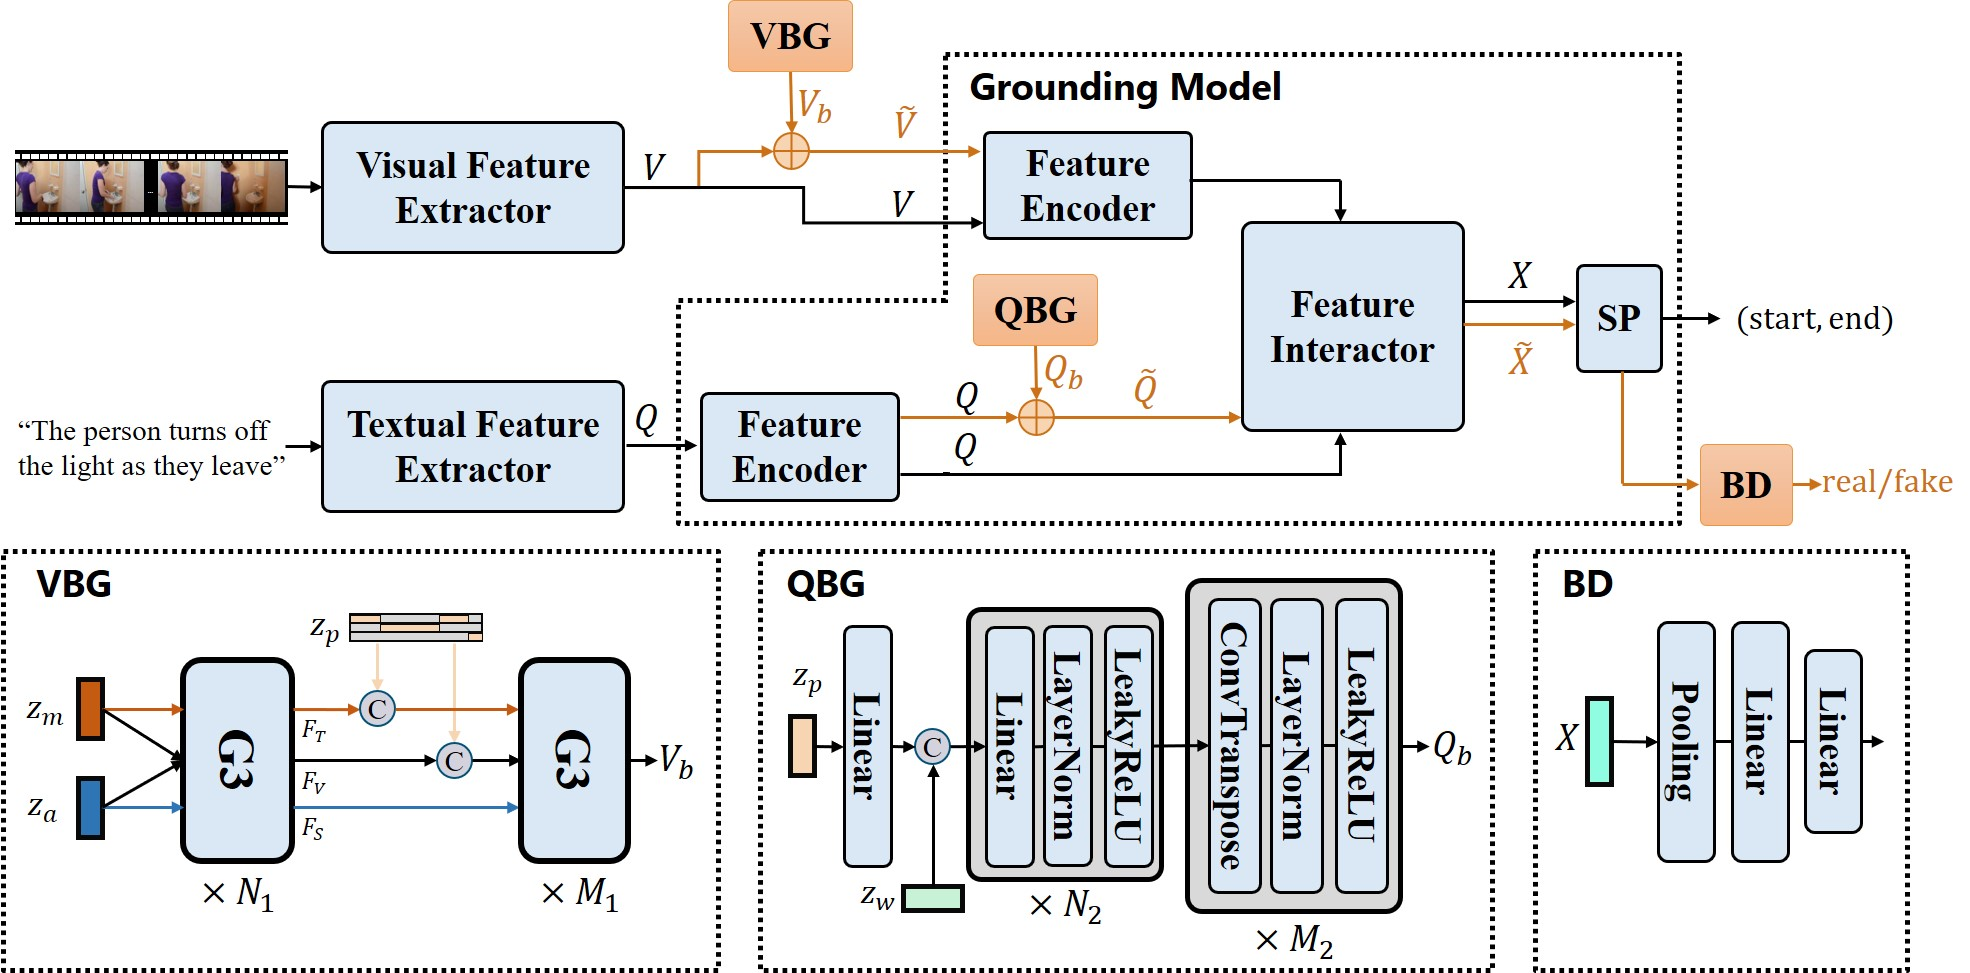
\includegraphics[width=0.96\linewidth]{images/OverView.jpg}%-crop.pdf}
	\caption{An overview of our BSSARD. The orange background is only used during the training period. Best viewed in color.}
	%\vspace{-3mm}
	\label{Overview}
\end{figure*}


\section{Method}


\subsection{Overview}

Our bias-conflict sample synthesis and adversarial removal debias strategy (BSSARD) is shown in Figure~\ref{Overview}, which is based on a span-based grounding model and incorporates a Visual Bias Generator (VBG), a Query Bias Generator (QBG), and a Bias Discriminator (BD). 

In the training stage, given a video-query pair~$(I_v,I_q)$ with the target moment~$(y_s^r,y_e^r)$ , we first utilize the visual and textual feature extractor to capture feature representations $V$ and $Q$. 
On the one hand, we feed the original $V$ and $Q$ into the feature encoder and feature interactor to obtain real sample feature $X$. Then, the span predictor (SP) should accurately produce the start and end time of the target moment. Meanwhile, the bias discriminator module should accurately predict it as the real sample. 
On the other hand, given a fake temporal location $z_p=(y_s^f, y_e^f)$ of the target moment obtained through random uniform sampling from the video frames, we employ VBG to generate visual bias feature $V_b$ and element-wise add it to the real sample feature $V$, which produces $\tilde{V}$. Similar to the real sample, we obtain bias-conflict sample feature $\tilde{X}$. It has two labels, one is the temporal position $(y_s^r,y_e^r)$ of the real target moment and the other is the fake temporal position $(y_s^f, y_e^f)$. The bias generator wants to generate shortcut features to trick SP into generating a target moment similar to $z_p$ and trick BD into judging the current sample as the real sample. Instead, the SP will try to generate target moments as close as $(y_s^r,y_e^r)$ and the BD will judge it as a sample with bias. 
Similarly, we also employ QBG to generate textual bias feature $Q_b$ and perform the above process. 
The synthesized bias features simulate all kinds of spurious correlations between the semantic information of video/text and the temporal position of the target clips. Through adversarial training, it effectively mitigates visual and linguistic biases. 
In the inference stage, the VBG, QBG, and BD components are removed. 


\subsection{Bias Generator}
% We implement a visual bias generator and a query bias generator to model visual bias and language bias respectively. 
%is a conditional generator that 

The bias generator generates bias-conflict sample features based on synthesized spurious relationships between the unimodality information and the temporal positional labels. 


\subsubsection{Visual Bias Generator} 

We construct VBG by the $\text{G}^\text{3}$ module~\cite{G3AN}, which encodes video features by decoupling appearance and motion content. The VBG contains three randomly generated variables $z_a$, $z_m$, and $z_p$ as inputs, and generates visual bias vector $V_{b}$ for constructing bias-conflict samples. These random variables guarantee the diversity and randomness of the bias generator.

Especially, the $z_a$ and $z_m$ are random vectors that follow a normal distribution and represent appearance and motion content, respectively. 
VBG first inputs $z_a$ and $z_m$ into $N_1$ stacked $\text{G}^\text{3}$, and produces three visual stream features, named temporal stream $F_T$, spatial stream $F_S$ and video stream $F_V$. 
Then, we random generate a fake temporal label $z_p \in \mathbb{R}^{3 \times n}$ of the target clip, which is obtained through random uniform sampling from the video frame sequence within the range of $\left[0, n-1\right]$. Its three dimensions are mutually exclusive and represent whether the segment contains background, foreground, or ignored data. It provides the temporal position conditional information that the bias generator requires. Subsequently, $z_p$ is concatenated with $F_T$ and $F_V$ to introduce temporal position information. 
Next, VBG outputs the visual bias vector $V_b\in \mathbb{R}^{n \times d}$ through $M_1$ stacked $\text{G}^\text{3}$. Finally, we add $V_b$ to $V$ and obtain visual bias conflict sample feature $\tilde{V}$,
\begin{equation}
	\begin{split}
		V_{b} &= VBG\left(z_a, z_m, z_p\right)\\
		\tilde{V} &= V_b + V
	\end{split}	
	\label{eq1}
\end{equation}
where $n$ and $d$ are the video length and feature dimension.


\subsubsection{Query Bias Generator}

We construct QBG by a simple fully connected structure and transpose convolutional structure. 
The QBG needs two randomly generated variables $z_w$ and $z_p$ as inputs and generates textual bias vector $Q_{b}$ for constructing bias-conflict samples. 

Specifically, we randomly sample $z_p$ from a normal distribution, which is a random vector of length $n$ and represents the synthetic label of the fake target video moment. Then we embed it using a fully connected layer, which provides the temporal position information for the feature generation. 
To enhance randomness and diversity, QBG also generates a random vector $z_w$ from a normal distribution to introduce the context for the feature generation, which is concatenated with the encoded position feature. 
We use $N_2$ linear layers and $M_2$ transposed convolution layers to produce the word sequence bias feature $Q_b\in \mathbb{R}^{m \times d}$. Finally, we add $Q_b$ to $Q$ and obtain query bias conflict sample feature $\tilde{Q}$,
\begin{equation}
	\begin{split}
		Q_b &= QBG\left(z_w, z_p\right)\\ 
		\tilde{Q} &= Q_b + Q
	\end{split}
	\label{eq2}
\end{equation}
where $m$ represents the length of the query text.


\subsection{Grounding Model}

The grounding model consists of a feature encoder, feature interactor, span predictor (SP), and bias discriminator (BD). 
BD is a binary classifier that identifies whether the sample contains biases. 
SP should make correct temporal grounding predictions for both regular and bias-conflict samples. 

For the normal samples without synthetic bias features, $V$ and $Q$ are encoded by the feature encoder and feature interactors to generate cross-modal representations $X$. Subsequently, the SP and BD make predictions, 
\begin{equation}
	\begin{split}
		p_{s}^r, p_{e}^r &= SP(X) \in \mathbb{R}^{n}, \mathbb{R}^{n}\\
		p_{d}^r &= BD(X) \in \mathbb{R}^{2}
	\end{split}
	\label{eq3}
\end{equation}
where $p_{s}^r$ and $p_{e}^r$ represent the predicted start and end positions of the target moment for the real sample, and $p_{d}^r$ represents the probability of the sample containing bias.

For bias-conflict samples, we iteratively encode $\tilde{V}$ and $Q$ or $V$ and $\tilde{Q}$ in each training iteration by the feature encoder and feature interactor to generate cross-modal representation $\tilde{X}$. Subsequently, the SP and BD make predictions,
\begin{equation}
	\begin{split}
		p_{s}^f, p_{e}^f &= SP(\tilde{X}) \in \mathbb{R}^{n}, \mathbb{R}^{n}\\
		p_{d}^f &= BD(\tilde{X}) \in \mathbb{R}^{2}
	\end{split}
	\label{eq4}
\end{equation}
where $p_{s}^f$ and $p_{e}^f$ represent the predicted start and end positions of the target moment for the bias-conflict sample, and $p_{d}^f$ represents the probability of the sample containing bias.


\subsection{Training Objectives}

\subsubsection{Training Process}

As shown in Algorithm~\ref{Training Process}, we train the two bias generators alternately in each training step. We detail the bias generator loss $L^g$ and the discriminator loss $L^d$.


\begin{algorithm}[t]
	\caption{Training process in one epoch.}
	\label{Training Process}
	\begin{algorithmic}[1] %这个1 表示每一行都显示数字
		\REQUIRE $\text{VBG}$; $\text{QBG}$; $\text{GD}$;
		\ENSURE TSGV model
		\FOR{each training iteration}
		\STATE Sample $\left(V, Q \right)$, $(y_s^r,y_e^r)$
		\STATE Sample $z_m$, $z_a$, $z_p$, $(y_s^f,y_e^f)$
		\STATE $V_b \leftarrow \text{VBG}(z_m, z_a, z_p)$
		\STATE $\tilde{V} \leftarrow V + V_b$, $\tilde{Q} \leftarrow Q$
		\STATE Get $p_{s}^r, p_{e}^r, p_{d}^r, p_{s}^f, p_{e}^f, p_{d}^f$ by Equation~\ref{eq3} and~\ref{eq4} 
		\STATE Calculate $L^g$ and train VBG, freeze GD
		\STATE Calculate $L^d$ and train GD, freeze VBG
		
		\STATE Sample $z_w$, $z_p$, $(y_s^f,y_e^f)$
		\STATE $Q_b \leftarrow \text{QBG}(z_w, z_p)$
		\STATE $\tilde{V} \leftarrow V$, $\tilde{Q} \leftarrow Q + Q_b$
		\STATE Get $p_{s}^r, p_{e}^r, p_{d}^r, p_{s}^f, p_{e}^f, p_{d}^f$ by Equation~\ref{eq3} and~\ref{eq4} 
		\STATE Calculate $L^g$ and train QBG, freeze GD
		\STATE Calculate $L^d$ and train GD, freeze QBG
		\ENDFOR
	\end{algorithmic}
\end{algorithm}


\subsubsection{Bias Generator Training Objectives}
The visual/query bias generator aims to deceive the bias discriminator and induce the span predictor to produce the given fake labels.

We use cross-entropy loss to trick the bias discriminator,
\begin{equation}
	L_{cls}^g=f_{CE}(p_{d}^f, 0)
	\label{g_loss_cls}
\end{equation}
where $p_d^f$ represents the predicted sample flag. $0$ indicates the current sample is a real sample without synthetic bias. It encourages the generator to generate samples that the BD will classify as unbiased. 

To induce span predictor, we use cross-entropy loss:
\begin{equation}
	L_{loc}^g=\frac{1}{2}\left[f_{CE}\left(p_{s}^{f}, y_{s}^{f}\right)+f_{CE}\left(p_{e}^{f}, y_{e}^{f}\right)\right]
	\label{g_loss_loc}
\end{equation}
This encourages the bias generator to generate bias-conflict samples that can deceive the grounding model.

The total training loss of the bias generator is
\begin{equation}
	L^{g}=L_{loc}^g+\lambda_{1} L_{cls}^g
	\label{g_loss}
\end{equation}
where $\lambda_{1}$ is a weight hyperparameter.


\subsubsection{Discriminator Training Objectives}
The discriminator needs to distinguish between real and bias-conflict samples and predict the true target moments.

For the bias discriminator, we use cross-entropy loss,
\begin{equation}
	L_{cls}^d=f_{CE}(p_{d}^r, 0) + f_{CE}(p_{d}^f, 1)
	\label{d_loss_cls}
\end{equation}
It encourages the discriminator to accurately judge real and synthetic samples.

For the temporal grounding, we use the traditional span-based cross-entropy loss,
\begin{equation}
	\begin{split}
		L_{loc}^d =&\frac{1}{2}\left[f_{CE}\left(p_{s}^{r}, y_{s}^{r}\right)+f_{CE}\left(p_{e}^{r}, y_{e}^{r}\right)\right]\\
		+& \frac{1}{2}\left[f_{CE}\left(p_{s}^{f}, y_{s}^{r}\right)+f_{CE}\left(p_{e}^{f}, y_{e}^{r}\right)\right]\\
	\end{split}
	\label{d_loss_loc}
\end{equation}

Besides, we find it advantageous to incorporate a sample-based distance metric such as KL divergence. Consequently, we introduce an additional objective, 
\begin{equation}
	L^d_{kl} = D_{kl}(p_{s}^{r} \| p_{s}^{f}) + D_{kl}(p_{e}^{r} \| p_{e}^{f})
	\label{loss_kl_d}
\end{equation}
Here, Equation~\ref{d_loss_loc} aligns the predictions towards the real labels, and Equation~\ref{loss_kl_d} limits the predictions of bias-conflict samples to not deviate much from the predictions of the corresponding original samples. 
Meanwhile, KL divergence is a regularization method to prevent the generator from overfitting training data and improve the generalization ability. 


\begin{table*}[t]
	\centering
	% \small
	\renewcommand{\arraystretch}{1}
	\setlength{\tabcolsep}{1.4mm}
	\begin{tabular}{c c c c | c c c|c c c | c c c}
		\toprule
		\multirow{3}{*}{Method}
		& \multicolumn{6}{c}{Charades-CD} & \multicolumn{6}{c}{ActivityNet-CD} \\
		& \multicolumn{3}{c}{OOD} & \multicolumn{3}{c}{IID} & \multicolumn{3}{c}{OOD} & \multicolumn{3}{c}{IID}\\
		& r1i5 & r1i7 & mIoU & r1i5 & r1i7 & mIoU & r1i5 & r1i7 & mIoU & r1i5 & r1i7 & mIoU \\
		\midrule
		2D-TAN~\cite{RN2} & 28.18 & 13.73 & 34.22 & 46.48 & 28.76 & 42.73 & 18.86 & 9.77 & 28.31 & 40.87 & 28.95 & 44.99\\
		
		LG~\cite{RN21} & 42.90 & 19.29 & 39.43 & 51.28 & 28.68 & 45.16 &
		23.85 & 10.96 & 28.46 & 46.41 & 29.28 & 44.62\\
		
		DRN~\cite{RN20} & 31.11 & 15.17 & 23.05 & 42.04 & 23.32 & 28.21 & 
		- & - & - & - & - & -\\
		
		VSLNet~\cite{RN4} & 34.10 & 17.87 & 36.34 & 43.26 & 28.43 & 42.92 &
		20.03 & 10.29 & 28.18 & 47.81 & 29.07 & 46.33\\
		
		DCM~\cite{RN29} & 40.51 & 21.02 & 40.99 & 52.50 & 35.28 & 48.74 & 20.86 & 11.07 & 28.08 & 42.15 & 29.69 & 45.20\\
		
		SVTG~\cite{RN30} & 46.67 & 27.08 & 44.30 & 57.59 & 37.79 & 50.93 &
		24.57 & 13.21 & 30.45 & 48.07 & 32.15 & 47.03\\
		
		MDD~\cite{lan2022closer} & 40.39 & 22.70 & - & 52.78 & 34.71 & - & 20.80 & 11.66 & - & 43.63 & 31.44 & - \\
		
		\midrule
		QAVE~\cite{hao2022query} & 37.84 & 19.67 & 38.45 & 47.63 & 29.28 & 44.17 &
		21.39 & 10.86 & 28.41 & 44.58 & 27.42 & 44.28 \\
		
		BSSARD-QAVE & \bf 44.47 & \bf 26.16 & \bf 42.95 & \bf 54.31 & \bf 37.67 & \bf 49.41 & \bf 23.11 & \bf 12.17 &	\bf 29.40 & \bf 46.04 & \bf 30.06 & \bf 45.56 \\
		
		\midrule
		EXCL~\cite{RN3} & 39.61 & 19.35 & 38.81 & 47.18 & 26.59 & 44.02 & 23.38 & 12.66 &	29.19 & 45.76 & 29.62 & \bf 46.42 \\
		BSSARD-EXCL &  {\bf 41.93} & {\bf 22.53} & {\bf 40.9} & \bf 50.00 & \bf 31.86 & \bf 46.47 & \bf 23.75 & \bf 12.93 & \bf 29.26 & \bf 46.98 & \bf 30.34 & 46.12 \\
		
		\midrule
		VSLNet*~\cite{RN4} & 43.08 & 22.52 & 41.52 & 52.86 & 34.87 &  48.23 &
		25.40 & 13.51 & 30.33 & 48.07 & 31.19 & 46.94\\
		BSSARD-VSLNet* & {\bf 47.20} & {\bf 27.17} & {\bf 44.59} & {\bf 55.65} & {\bf 36.33} & {\bf 50.45} &
		{\bf 27.02} & {\bf 14.93} & {\bf 31.49} & {\bf 49.67} & {\bf 33.72} & {\bf 48.54}\\
		
		\bottomrule
	\end{tabular}
	\caption{Comparison results with state-of-the-arts. VSLNet*	replaces the encoder in VSLNet with a transformer block.}
	\label{sota-redivided}
\end{table*}


The total training loss of the discriminator is:
\begin{equation}
	L^d=L_{loc}^d+\lambda_{2} L_{cls}^d + \lambda_{3} L_{kl}^d
	\label{eq12}
\end{equation}
where $\lambda_{2}$ and $\lambda_{3}$ are weight hyperparameters.


\section{Experiment}

\subsection{Experiment Setup}

\subsubsection{Datasets}

We conduct experiments on the repartitioned Charades-CD and ActivityNet-CD~\cite{lan2022closer}. 
In these repartitioned datasets, the target moments of samples in the training, val, and test-iid sets are independent and identically distributed, while the test-ood set contains out-of-distribution samples. 
We can verify the debias ability of different models according to the grounding performance on the test-ood set and the performance difference between test-iid and test-ood sets.


\subsubsection{Metrics}
We use evaluation metrics of R@$n$, IoU=$m$, and mIoU. 
R@$n$, IoU=$m$ measures the proportion of test samples in which at least one of the top-$n$ localization results has an IoU score greater than $m$. 
The mIoU measures the average IoU score across all test samples. 
We set $n$ to 1 and $m$ to either 0.5 or 0.7, and use r1i5 and r1i7 to denote R@1, IoU=0.5 and R@1, IoU=0.7, respectively.
% We utilized the evaluation metrics of R$@n$, IoU=$m$ and mIoU. R$@n$, IoU=$m$ measures the percentage of testing samples with at least one localized result in the top-$n$ that has an IoU score greater than $m$ with the ground truth. On the other hand, mIoU measures the average IoU score across all testing samples. We use $n = 1$ and $m \in \{0.5,0.7\}$ in our experiments. We use r1i5 and r1i7 to respectively denote R@1, IoU=0.5 and R@1, IoU=0.7.


\subsubsection{Implementation Details}
For the text feature extractor, we use 300d GloVe~\cite{Glove} vectors for initialization. For the visual feature extractor, we use pre-trained I3D~\cite{I3D} and C3D~\cite{C3D} features. For the visual bias generator, we set $N_1$ to 4 and $M_1$ to 2. For the query bias generator, we set $N_2$ to 2 and $M_2$ to 4. During the training process, we use the AdamW~\cite{AdamW} optimizer, with a batch size of 16, and an initial learning rate of 0.001. We set $\lambda_{1}$ to 1, $\lambda_{2}$ to 1, and $\lambda_{3}$ to 1. 


\begin{table}[t]
	\centering
	% \small
	\renewcommand{\arraystretch}{1}
	\setlength{\tabcolsep}{1mm}
	\begin{tabular}{c|cc|ccc|ccc}
		% \hline
		\toprule
		\multirow{2}{*}{Row}
		& \multicolumn{2}{c}{BG} & \multicolumn{3}{c}{Grounding} &
		\multicolumn{3}{c}{OOD}  \\
		& $L_{loc}^g$ & $L_{cls}^g$ & $L_{loc}^d$ & $L_{cls}^d$ & $L_{kl}^d$
		& r1i5 & r1i7 & mIoU \\
		% \specialrule{1.5pt}{0em}{0em}
		\midrule
		1 & - & - & $\checkmark$ & - & - &
		43.08 & 22.52 & 41.52 \\
		2 & $\checkmark$ & - & $\checkmark$ & - & - &
		46.64 & 26.40 & 43.49 \\
		3 & $\checkmark$ & - & $\checkmark$ & - & $\checkmark$ &
		45.99 & 26.16 & 44.02 \\
		4 & - & $\checkmark$ & $\checkmark$ & $\checkmark$ & - &
		45.16 & 25.72 & 43.18 \\
		5 & - & $\checkmark$ & $\checkmark$ & $\checkmark$ & $\checkmark$ & 
		46.22 & 26.40 & 44.22 \\
		6 & $\checkmark$ & $\checkmark$ & $\checkmark$ & $\checkmark$ & - & 
		{\bf 47.41} & 26.84 & 44.00 \\
		7 & $\checkmark$ & $\checkmark$ & $\checkmark$ & $\checkmark$ & $\checkmark$ &
		47.20 & {\bf 27.17} & {\bf 44.59} \\
		\bottomrule
	\end{tabular}
	\caption{Ablation study about loss functions.}
	\label{loss term study}
	%\vspace{-3mm}
\end{table}


\subsection{Comparison with State-of-the-Arts}

To verify the universality of our debias strategy, we implement our BSSARD on multiple existing backbones QAVE, ExCL, and VSLNet*. The experiment results on Charades-CD and ActivityNet-CD datasets are presented in Table~\ref{sota-redivided}. 
We can see that our approach can significantly improve the grounding performance of different backbones on most evaluation metrics for OOD and IID test sets in both datasets. This indicates that our method has stronger debias and grounding ability. 
Besides, although our method shows the best performance in ActivityNet-CD's IID (BSSARD-VSLNet*), it works weaker than SVTG in Charades-CD's IID test set. This is due to the IID test set of Charades-CD containing a higher proportion of biased samples. 
% For example, in Charades-CD, our method achieves 4.12\% and 2.79\% for IoU=0.5, and 4.65\% and 1.46\% for IoU=0.7, respectively. Similarly, in ActivityNet-CD, our method achieves 1.62\% and 1.6\% for IoU=0.5, and 1.72\% and 2.53\% for IoU=0.7, respectively. 


\subsection{Ablation Study}

We conduct abundant ablation studies on Charades-CD datasets over BSSARD-VSLNet* backbones. 

\subsubsection{Loss Terms}

We analyze the impact of each loss function and their combinations on the grounding performance. Table~\ref{loss term study} summarizes the results. 
We can see that each loss function has its validity, and the combination of generation and adversarial losses can further improve the grounding performance on the OOD test set. 
Besides, the $L_{kl}^d$ leads to performance improvements in most cases. However, the improvement is limited when $L_{cls}^d$ is not used. This is because $L_{kl}^d$ depends on the grounding model's attention to the bias features brought by $L_{cls}^d$.


\begin{table}[t]
	\centering
	%\small
	\renewcommand{\arraystretch}{1}
	\setlength{\tabcolsep}{0.4mm}
	\begin{tabular}{c c c c | c c c}
		\toprule
		\multirow{2}{*}{Method} & \multicolumn{3}{c}{OOD} & \multicolumn{3}{c}{IID}\\
		& r1i5 & r1i7 & mIoU & r1i5 & r1i7 & mIoU \\
		\midrule
		%		QAVE &    &    &    &    &    &    \\
		%		QAVE-Q &    &    &    &    &    &    \\
		%		QAVE-V &    &    &    &    &    &    \\
		%		ADTGN-QAVE &    &    &    &    &    &    \\
		QAVE & 37.84 & 19.67 & 38.45 & 47.63 & 29.28 & 44.17 \\
		QAVE-Q & 41.96 & 23.20 & 40.97 & 50.18 & 32.56 & 47.11 \\
		QAVE-V & 42.79 & 22.34 & 41.03 & 54.07 & 33.41 & 48.31 \\
		BSSARD-QAVE & \bf 44.47 & \bf 26.16 & \bf 42.95 & \bf 54.31 & \bf 37.67 & \bf 49.41 \\
		\midrule
		ExCL & 39.61 & 19.35 & 38.81 & 47.18 & 26.59 & 44.02\\
		ExCL-Q & 39.94 & 19.7 & 39.05 & 48.90 & 26.59 & 44.72 \\
		ExCL-V & 39.10 & 19.21 & 38.77 & 47.79 & 30.76 &  45.58 \\
		BSSARD-ExCL & {\bf 41.93} & {\bf 22.53} & {\bf 40.9} & \bf 50.00 & \bf 31.86 & \bf 46.47 \\
		\midrule
		VSLNet* & 43.08 & 22.52 & 41.52 & 52.86 & 34.87 &  48.23 \\	
		VSLNet*-Q & 44.86 & 25.30 & 42.91 & 53.10 & 33.78 & 49.13 \\
		VSLNet*-V & 45.16 & 25.48 & 44.04 & {\bf 55.89} & {\bf 36.57} &  {\bf 51.60}\\
		BSSARD-VSLNet* & {\bf 47.20} & {\bf 27.17} & {\bf 44.59} & 55.65 & 36.33 & 50.45 \\
		\bottomrule
	\end{tabular}
	\caption{Ablation study about bias generator.}
	\label{backbones_charades_cd}
	%\vspace{-3mm}
\end{table}


\begin{table}[t]
	\centering
	\renewcommand{\arraystretch}{1}
	\begin{tabular}{c c c c c}
		\toprule
		visual & language & r1i5 & r1i7 & mIoU\\
		\midrule
		before & before & {\bf 47.32} & 26.46 & 44.30 \\
		before & after & 47.20 & {\bf 27.17} & {\bf 44.59} \\
		after & before & 45.45 & 25.30 & 42.66 \\
		after & after & 46.67 & 25.90 & 43.69 \\
		\bottomrule
	\end{tabular}
	\caption{Ablation study about bias injection positions. ``before'' and ``after'' represent the injection position before and after the feature encoder, respectively.}
	\label{bias_injection_positions}
\end{table}


\subsubsection{Bias Generator}

We analyze the impact of visual and query bias generators on different backbones and show the results in Tables~\ref{backbones_charades_cd}.
*-V and *-Q refer to the backbone model that uses only visual and query bias generators, respectively. The results show that the visual and query bias generators are effective on all backbones, and the two generators complement each other. 
Besides, we find that the performance of VSLNet*-V is even better than BSSARD-VSLNet* on the IID test set. This is mainly due to two reasons, one is that the powerful cross-modality alignment ability of VSLNet* weakens the integration effect of the two bias generators, and the other is the presence of numerous language bias samples in the IID test set.


\subsubsection{Bias Injection Positions}

We explore the effect of bias feature injection positions. 
The injection position determines which features the bias generator needs to generate bias on and which parts of the grounding model need to complete debias task. 
For visual and language biases, we separately test the injection position before and after the feature encoder. The results are shown in Table~\ref{bias_injection_positions}. 
We can see that injecting the visual bias feature before the visual feature encoder and injecting the language bias feature after the language feature encoder is the most effective. 
This primarily depends on the distinct characteristics of vision and text data and the need for both accuracy and diversity in generated bias features. First, the intricate nature of video content
and the high-dimensional visual feature space pose serious challenges for the feature encoder that aims to map visual and textual features into a shared space for multi-modal feature alignment. Injecting visual bias before the feature encoder reduces the encoder’s learning complexity, enabling the model to differentiate real from synthesized visual features. Second, introducing language bias after the feature encoder helps the model better capture bias during the multimodal feature alignment stage. Third, multiple injection positions increase the diversity of generated bias features. 

Besides, we inject bias in the feature domain instead of the input data because it is more controllable to generate high-quality sample features. If we directly generate video samples, the generator should not only capture the bias information but also learn the original video representation, which greatly increases the learning difficulty. %Moreover, we use the pre-trained models with fixed parameters to extract features, which can preserve rich relationships in the data domain in the feature space. 


\begin{table}[t]
	\centering
	\renewcommand{\arraystretch}{1}
	\begin{tabular}{c c c c c}
		\toprule
		$z_p$ & concat & r1i5 & r1i7 & mIoU\\
		% Fusion method & r1i5 & r1i7 & mIoU\\
		\midrule
		$\mathbb{R}^{n}$ & $F_T,F_V$ & 46.40 & 26.40 & 44.07 \\
		
		$\mathbb{R}^{3 \times n}$ & $F_T,F_V$ & {\bf 47.20} & {\bf 27.17} & {\bf 44.59}\\
		
		$\mathbb{R}^{3 \times n}$ & $F_T,F_V,F_S$ & 46.70 & 26.28 & 44.15 \\
		
		\bottomrule
	\end{tabular}
	\caption{Ablation study about fusion method of $z_p$.}
	\label{fusion method}
\end{table}


\begin{table}
	\centering
	\renewcommand{\arraystretch}{1}
	\setlength{\tabcolsep}{2mm}
	\begin{tabular}{c c c c}
		\toprule
		Training strategy & r1i5 & r1i7 & mIoU \\
		\midrule
		alternate each epoch & 46.79 & 26.76 & 44.53 \\
		
		random each step & 45.81 & 25.84 & 43.81 \\
		
		alternate each step & {\bf 47.20} & {\bf 27.17} & {\bf 44.59}\\
		
		\bottomrule
	\end{tabular}
	\caption{Ablation study about training strategy.}
	\label{Training strategy}
\end{table}



\subsubsection{Fusion Method of $z_p$ in VBG}
We investigate the impact of different fusion methods between $z_p$ and visual features in VBG. 
Table~\ref{fusion method} summarizes the results on the OOD test set.
We test three fusion methods, 
(1) encoding the temporal position as $z_p \in \mathbb{R}^{n}$ and fusing it with the temporal stream $F_T$ and video stream $F_V$.
(2) encoding the temporal position as $z_p \in \mathbb{R}^{3 \times n}$ and fusing it with $F_T$ and $F_V$.
(3) encoding the temporal position as $z_p \in \mathbb{R}^{3 \times n}$ and fusing it with the $F_T$, $F_V$ and spatial stream $F_S$. 
The results demonstrate that the second method is the most effective.
This is because $z_p \in \mathbb{R}^{3 \times n}$ can better represent temporal position information, and only the time stream $F_T$ and video stream $F_V$ containing temporal information that can better utilize temporal position information.


\begin{figure*}[t]
	\centering
	\subfigure[``cook'' suggests the target moment starts at the video start.]{
		%\includegraphics[width=5cm]{images/motivation-case-1.jpg}
		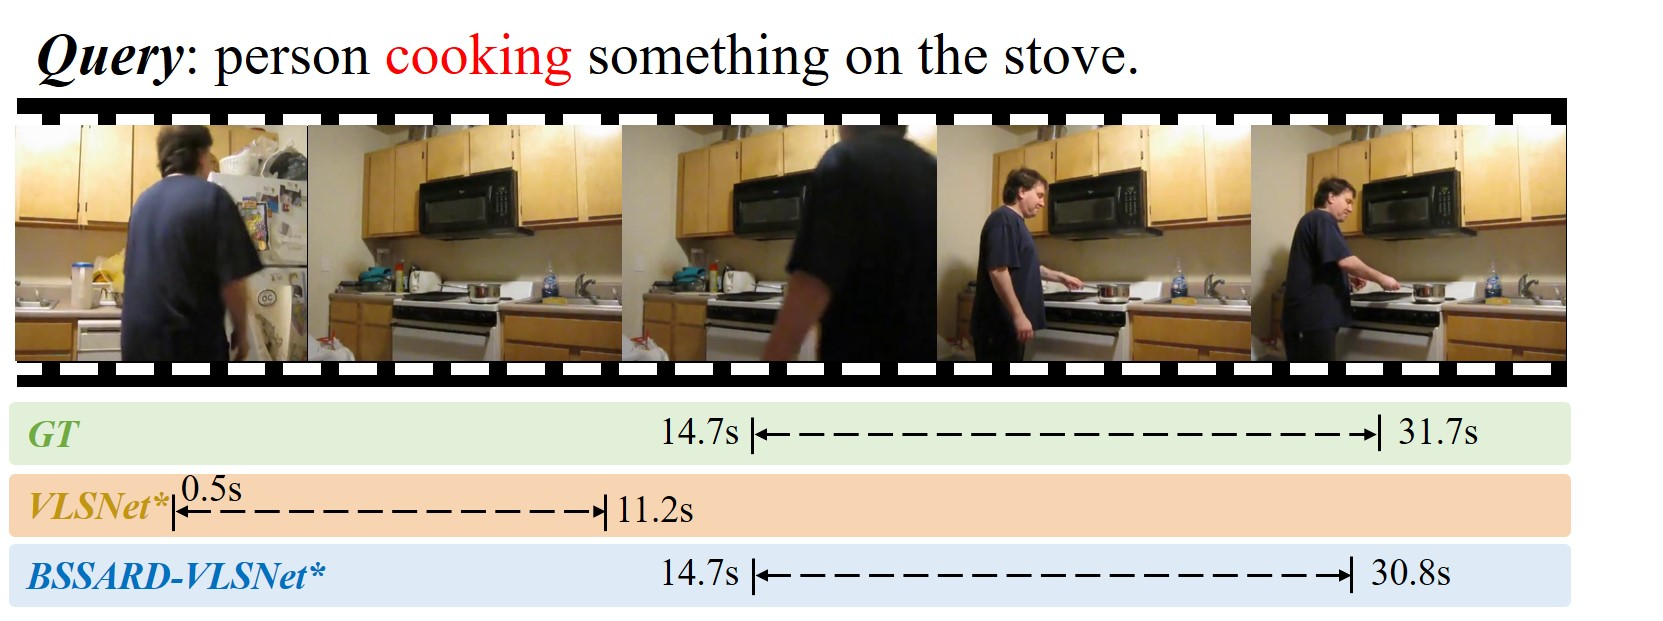
\includegraphics[scale=0.3]{images/cook.jpg}%-crop.pdf}
		\label{visualization_sample1}
	}
	\quad
	%\vspace{0.5mm}
	\subfigure[``start'' implies the target moment is at the end of the video.]{
		%\includegraphics[width=5cm]{images/motivation-case-2.jpg}
		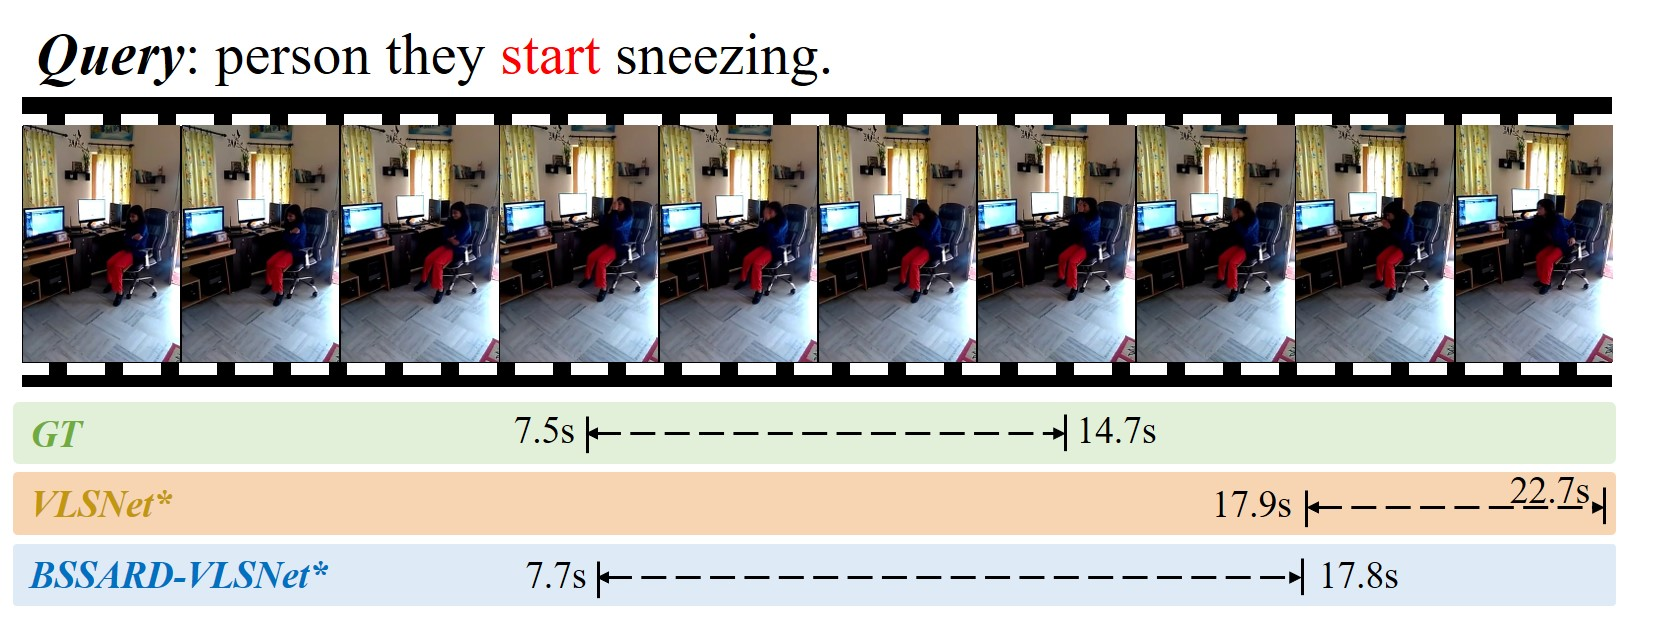
\includegraphics[scale=0.3]{images/start.jpg}%-crop.pdf}
		\label{visualization_sample2}
	}
	\quad
	\subfigure[``hold'' suggests the target moment starts at the video start.]{
		%\includegraphics[width=5cm]{images/motivation-case-3.jpg}
		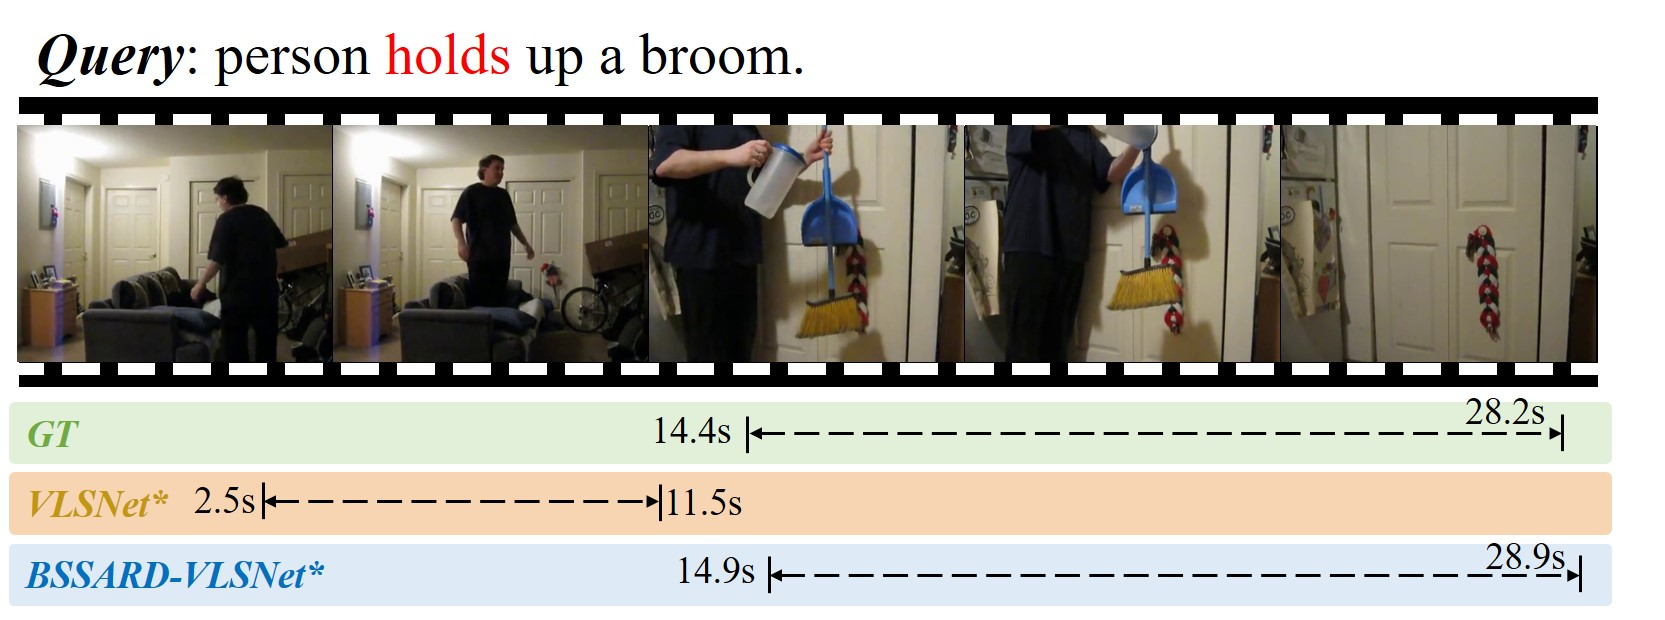
\includegraphics[scale=0.3]{images/hold.jpg}%-crop.pdf}
		\label{visualization_sample3}
	}
	\quad
	%\vspace{0.5mm}
	\subfigure[``hold'' suggests the target moment starts at the video start.]{
		%\includegraphics[width=5cm]{images/motivation-case-3.jpg}
		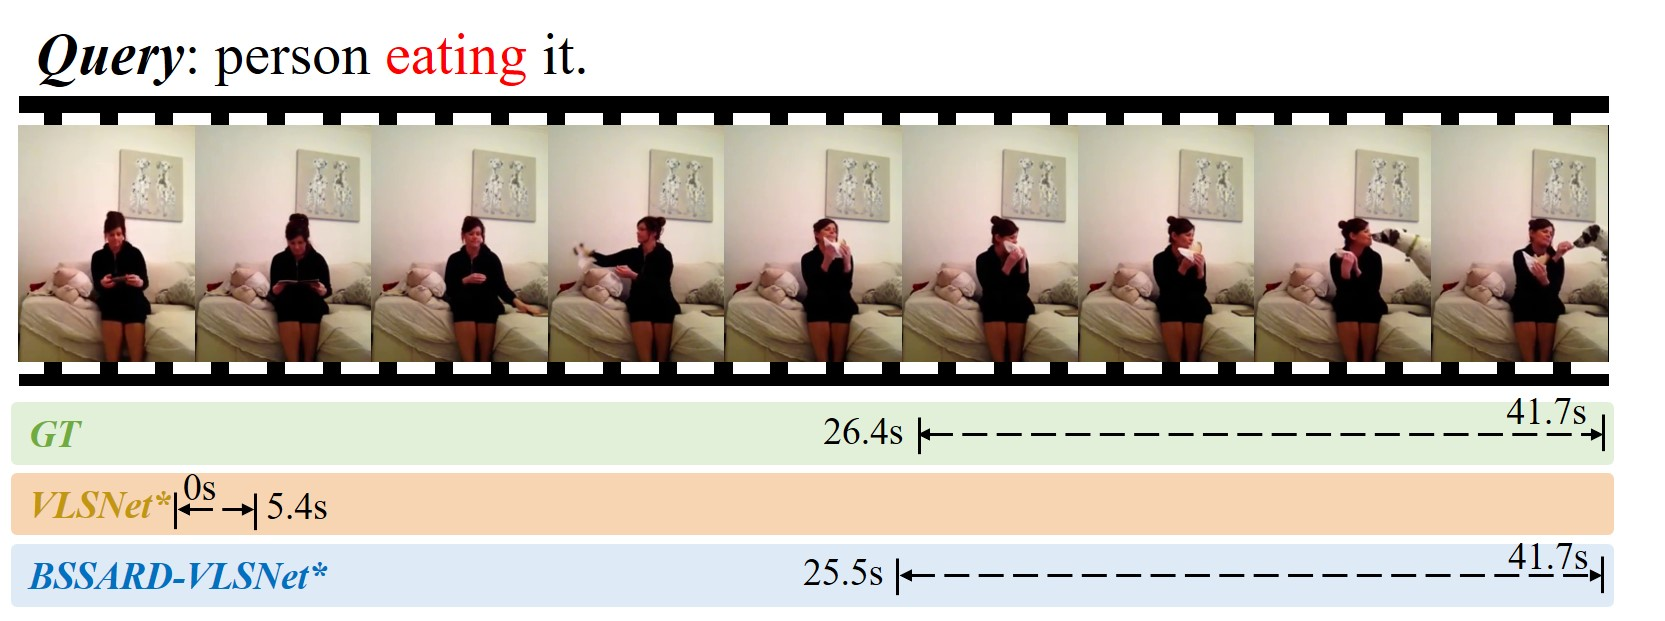
\includegraphics[scale=0.3]{images/eat.jpg}%-crop.pdf}
		\label{visualization_sample4}
	}
	\quad
	\centering
	\caption{The visualization comparison results between VLSNet* and BSSAR-VLSNet*.}
	\label{visualization_sample}
\end{figure*}


\subsubsection{Training Strategy for Bias Generators}
We investigate the impact of the training order of two bias generators and show results in Table~\ref{Training strategy}.
We test three training strategies: (1) alternately training the two bias generators at each epoch. (2) randomly selecting one bias generator for training at each training step. (3) alternately training the two bias generators at each training step. 
The experimental results indicate that the third training strategy is optimal. This is mainly because alternate training the two bias generators can avoid the model overfitting into a certain debias approach.


\subsection{Analysis of the Debias Effect}


\subsubsection{The Verification of Mitigating Bias} 

We randomly shuffle the words in each query text, which disrupts potential spurious correlations among query text and target moments. It also prevents the model from relying on visual-language alignment unless it depends on visual bias. Table~\ref{ablation_removing_language_bias} shows BSSARD achieves more significant performance degradation. This indicates our approach relies less on bias correlations beyond query text to perform grounding. 


\begin{table}[t]
	\centering
	\small
	\renewcommand{\arraystretch}{1}
	\setlength{\tabcolsep}{1.2mm}
	\begin{tabular}{c c c c c }
		\toprule
		Setting & B-VSLNet & VSLNet & B-QAVE & QAVE \\
		\midrule
		Original query & 47.20 & 43.08 & 44.47 & 37.84 \\
		%\midrule
		%Random video & 22.30 & 19.82 & 1.778 & 4.86 \\
		%Gap & \textbf{$\downarrow$ 52.75\%} & \textbf{$\downarrow$ 53.99\%} & \textbf{$\downarrow$ 96.00\%} & \textbf{$\downarrow$ 87.16\%} \\
		%\midrule
		Random query & 15.11 & 18.31 & 29.87 & 31.17 \\
		\midrule
		Gap & \textbf{67.99\% $\downarrow$ } & \textbf{57.50\% $\downarrow$} & \textbf{32.83\% $\downarrow$} & \textbf{17.63\% $\downarrow$} \\
		\bottomrule
	\end{tabular}
	\caption{Comparison results under random text input.}
	\label{ablation_removing_language_bias}
\end{table}


\subsubsection{Qualitative Analysis}

We also compare the debias effect of our BSSARD-VLSNet* and VLSNet* at the sample level in Figure~\ref{visualization_sample}. 
First, we give the temporal distribution of the target moment for samples with common verbs in the Charades-CD training set in Figure~\ref{sample_bias_distribution}. This indicates each verb contains prior knowledge for the localization of the target video clip. 
For example, the verb ``cook'' indicates that the temporal location of the target moments for most samples is the first half of the video. 
Hence, if the query text contains ``cook'' and the model will output the target moment with high probability in the first half of the video, which is the phenomenon of VLSNet* shown in Figure~\ref{visualization_sample1}. However, the result of our BSSARD-VLSNet* is not affected by the bias in the training set. 
The other three examples also show that the VLSNet* model relies on the bias in the training set for prediction, while our BSSARD-VLSNet* can effectively reduce the dependence on the bias and shift the model's attention back to cross-modality matching to make correct predictions. 


\begin{figure}[t]
	\centering
	{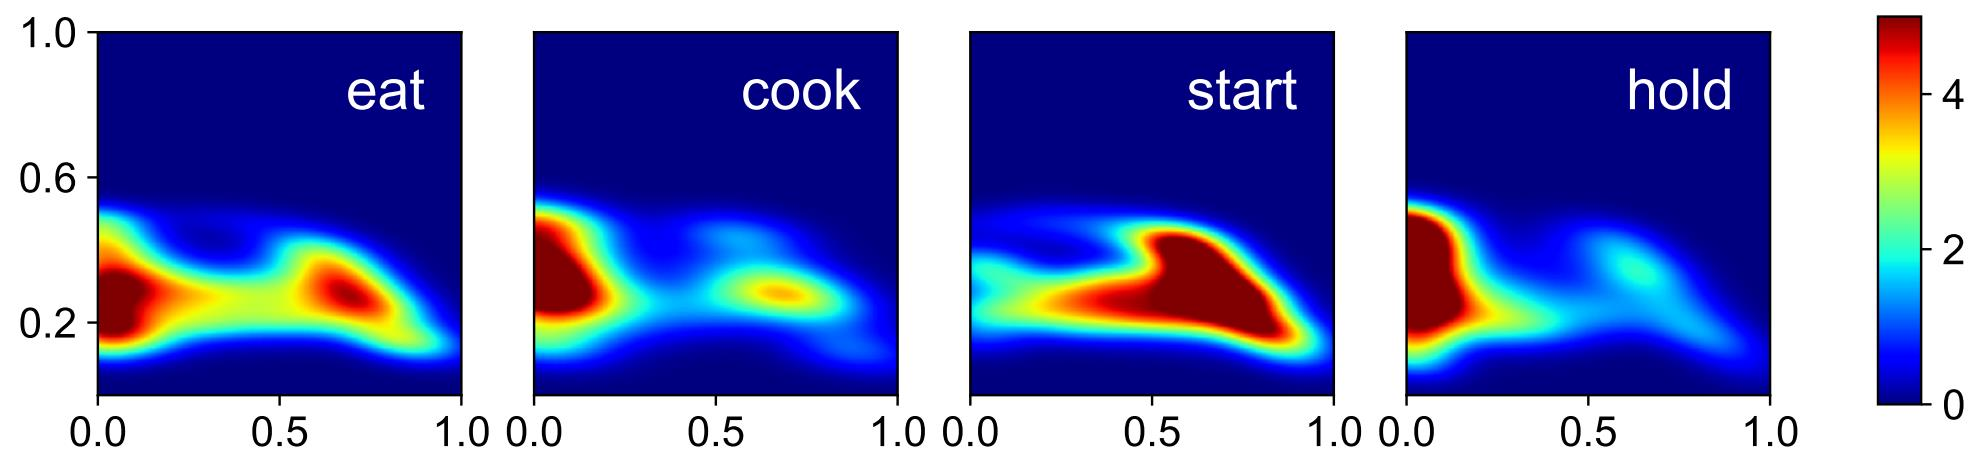
\includegraphics[width=1\linewidth]{images/distribution_four_word.jpg}}%.pdf}}
	\caption{The temporal distribution of target moments for video-text samples with certain common verbs. The horizontal and vertical axes denote the normalized starting time and duration of the target moment, respectively. The color represents the sample density.}
	\label{sample_bias_distribution}
\end{figure}




\section{Conclusion}
In this paper, we propose a novel adversarial training debias framework for TSGV task.
It dynamically generates bias-conflict samples by exploiting all kinds of spurious relationships between single-modality features and the target moments, which can effectively remove the bias dependency of the TSGV models.
In essence, the debias is achieved through directional data augmentation, which breaks the uneven temporal distribution of the target moments for samples that contain similar semantic components.
Extensive experiments on Charades-CD and ActivityNet-CD datasets demonstrate the effectiveness of our strategy.
In the future, we will apply our method to a wider range of scenarios, such as debias in visual question-answering task, and also eliminate cross-modality combination bias problems.



\section{Acknowledgments}
This work was supported in part by the National Natural Science Foundation of China under Grant U21B2038, 62306092, 61976069, 62022083, and 62236008.%, in part by the Research Start-Up Fund from Harbin Institute of Technology, Weihai under Grant IDGA10002144.



Vero modi repellendus eligendi, quaerat adipisci nobis accusamus maxime ex voluptatem laboriosam iure et nam, repellendus voluptatem quaerat reiciendis culpa distinctio optio, nisi illum dolor facilis nostrum accusamus, temporibus suscipit reprehenderit velit voluptatem.Perferendis animi reiciendis ea beatae possimus quia cupiditate quam quibusdam eveniet, inventore eum est quam, assumenda eaque officiis illo?Quod voluptates repellendus eius reiciendis aspernatur tempora assumenda, itaque dignissimos exercitationem?Eum nostrum eius aliquam doloremque veritatis laboriosam quisquam ipsum itaque, similique veritatis sed magni, quaerat mollitia ullam
\bibliography{aaai24}

\end{document}